\documentclass[11pt,a4paper]{article}
\usepackage[utf8]{inputenc}
\usepackage[T1]{fontenc}
\usepackage[spanish,es-noshorthands]{babel}
\usepackage{amsmath,amssymb,amsthm}
\usepackage{bm}
\usepackage{geometry}
\geometry{margin=2.5cm}
\usepackage{graphicx}
\graphicspath{{../figuras/}}
\usepackage{float}
\usepackage{xcolor}
\usepackage{hyperref}
\hypersetup{colorlinks=true,linkcolor=blue!50!black,citecolor=blue!50!black,urlcolor=blue!50!black}
\usepackage{enumitem}
\usepackage{booktabs}
\newtheorem{definition}{Definición}
\newtheorem{remark}{Observación}
\newcommand{\R}{\mathbb{R}}
\newcommand{\thetavec}{\bm{\theta}}
\newcommand{\transp}{^{\top}}
\newcommand{\promptIA}[1]{\begin{center}\fcolorbox{gray}{gray!8}{\parbox{0.9\linewidth}{\small\textbf{[FIGURA -- PROMPT IA]}\\[2pt]#1}}\end{center}}
\title{\textbf{B4 --- Ritmos cerebrales y acoplamiento theta--gamma}\\[2pt]\large Qué produce el modelo de Wilson--Cowan y por qué queremos controlarlo}
\author{Proyecto Wilson--Cowan --- Iniciación a la I+D ITBA}
\date{\today}
\begin{document}
\maketitle
\tableofcontents
\bigskip

Este documento continúa a \textbf{B3 (modelo de Wilson--Cowan)}. Allí vimos que el
sistema E--I, con los pesos y estímulos correctos, deja de relajar a un punto fijo y
entra en un \emph{ciclo límite}: una oscilación sostenida. Acá cambiamos de lente y
preguntamos: ¿qué representa biológicamente esa oscilación? La respuesta conecta a
Wilson--Cowan con los \emph{ritmos cerebrales} reales que se miden en EEG y LFP, y en
particular con el régimen \textbf{theta--gamma}, que es el objetivo de control de todo
el proyecto. La idea de fondo: si el modelo genera el mismo tipo de ritmo que produce
la corteza, entonces identificar sus parámetros (P1--P4) y luego controlarlo en lazo
cerrado tiene un sentido neurofisiológico concreto.

\section{Oscilaciones neuronales: las bandas clásicas}

Cuando registramos la actividad eléctrica de una población de neuronas, no vemos ruido
blanco: vemos energía concentrada en \emph{bandas de frecuencia}. Estas bandas se
definieron históricamente por inspección del EEG humano y hoy sabemos que cada una se
asocia (a grandes rasgos, con mucho solapamiento) a distintos estados y funciones.

\begin{definition}[Oscilación neuronal]
Fluctuación aproximadamente periódica de la actividad de una población de neuronas,
visible como energía concentrada alrededor de una frecuencia en el espectro de una
señal poblacional (EEG, LFP). No es una neurona ``marcando el ritmo'', sino un
comportamiento \emph{colectivo} de miles de células.
\end{definition}

\begin{center}
\begin{tabular}{@{}llp{7.2cm}@{}}
\toprule
\textbf{Banda} & \textbf{Rango aprox.} & \textbf{Asociación (a grandes rasgos)} \\
\midrule
Delta ($\delta$) & 0,5--4 Hz  & Sueño profundo (ondas lentas), estados de baja vigilancia. \\
Theta ($\theta$) & 4--8 Hz    & Memoria, navegación espacial, hipocampo; ritmo ``portador'' lento. \\
Alpha ($\alpha$) & 8--13 Hz   & Reposo con ojos cerrados, inhibición/desatención de regiones. \\
Beta ($\beta$)   & 13--30 Hz  & Estado de alerta, mantenimiento motor, control top--down. \\
Gamma ($\gamma$) & 30--80+ Hz & Procesamiento local activo, atención, ``binding'' perceptivo. \\
\bottomrule
\end{tabular}
\end{center}

\begin{remark}
Los límites exactos varían entre autores y no son fronteras físicas: una señal real
tiene potencia en todas las frecuencias y las bandas son ventanas convenientes. Lo
importante para nosotros es la relación de \emph{escalas de tiempo}: theta es lento
($\sim$100--250 ms por ciclo) y gamma es rápido ($\sim$12--30 ms por ciclo). Esa
separación de escalas es justo lo que hace posible el acoplamiento de la Sección~4.
\end{remark}

No tenemos una figura del espectro con las bandas en el paquete, así que dejamos el
placeholder para generarla:

\begin{figure}[H]\centering
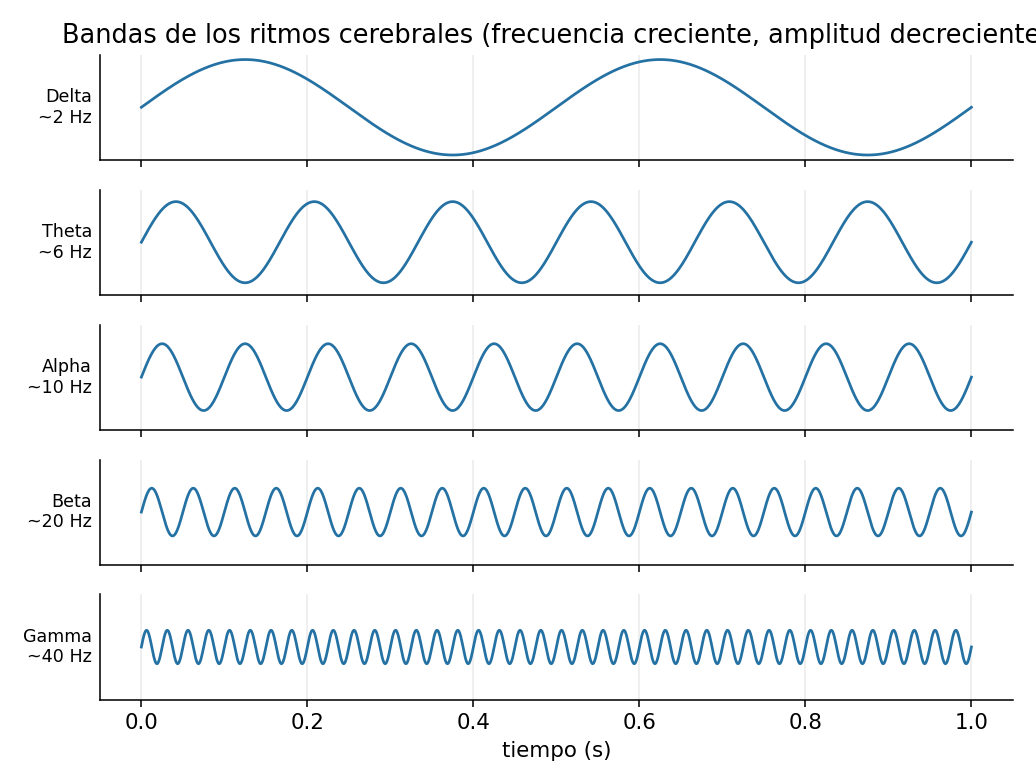
\includegraphics[width=0.8\linewidth]{fig_bandas_eeg.png}
\caption{Las cinco bandas clásicas de los ritmos cerebrales, cada una como una oscilación de ejemplo: a mayor frecuencia (delta $\to$ gamma), menor amplitud típica. En una señal de EEG/LFP real estas bandas coexisten superpuestas.}
\end{figure}

\section{Gamma: el mecanismo excitación--inhibición}

La banda gamma es especialmente relevante para nosotros porque su origen es
exactamente el mecanismo que modela Wilson--Cowan: la \textbf{interacción entre una
población excitatoria (E) y una inhibitoria (I)}.

La intuición del ``motor'' gamma es un lazo de retardo E$\to$I$\to$E:
\begin{enumerate}[nosep]
  \item Un pulso de actividad excitatoria (E$\uparrow$) recluta a las interneuronas
        inhibitorias (E$\to$I, peso $w_{IE}$).
  \item La inhibición sube (I$\uparrow$) y frena a E (I$\to$E, peso $w_{EI}$), con un
        retardo dado por la constante de tiempo $\tau_i$.
  \item Al caer E, cae también el reclutamiento de I; la inhibición decae y E puede
        volver a crecer.
\end{enumerate}
Ese ir y venir, con el desfasaje temporal entre excitación e inhibición, produce una
oscilación cuya frecuencia queda fijada por las constantes de tiempo y los pesos. Este
es, en la literatura, el mecanismo tipo \emph{PING} (pyramidal--interneuron network
gamma): la excitación dispara la inhibición y la inhibición apaga la excitación
ritmicamente \cite{buzsaki2012gamma}.

En términos del modelo (ver B3 para la derivación), las ecuaciones canónicas son
$$\dot I = \tfrac{1}{\tau_i}\big(-I + S_i(w_{IE}E - w_{II}I + Q(t) - \theta_i) - k_i\big),$$
$$\dot E = \tfrac{1}{\tau_e}\big(-E + S_e(w_{EE}E - w_{EI}I + P(t) - \theta_e) - k_e\big),$$
con $S_a(u)=1/(1+e^{-a u})$ y los offsets $k_e,k_i$ elegidos para que $E=I=0$ sea
equilibrio en reposo. El acoplamiento cruzado $w_{IE}$ (E excita a I) y $w_{EI}$ (I
frena a E) es exactamente el lazo E--I descrito arriba. Con los valores por defecto del
simulador ($w_{EE}{=}6{,}4$, $w_{EI}{=}4{,}8$, $w_{IE}{=}6{,}0$, $w_{II}{=}1{,}2$,
$\tau_e{=}1{,}0$, $\tau_i{=}2{,}0$) y una entrada adecuada (p.\,ej.\ $P\approx1{,}2$,
$Q\approx0{,}6$), el sistema tiene un ciclo límite estable: \textbf{Wilson--Cowan es un
generador de ritmo tipo gamma}. El período del ciclo, en las unidades adimensionales
del modelo, se lee como la ``frecuencia gamma'' de la población simulada.

\begin{remark}
Que $\tau_i > \tau_e$ (la inhibición es más lenta que la excitación) es lo que da el
retardo necesario para oscilar: si ambas respondieran instantáneamente, el sistema
relajaría directo al equilibrio. Cambiar $P,Q$ mueve al sistema entre un foco estable
(p.\,ej.\ $P{=}0{,}8$, $Q{=}0{,}6$: no oscila) y el ciclo límite ($P{=}1{,}2$,
$Q{=}0{,}6$: oscila). Esta sensibilidad al estímulo es la palanca que usará el
controlador.
\end{remark}

\section{Acoplamiento theta--gamma (\emph{cross-frequency coupling})}

Un solo ritmo gamma es solo la mitad de la historia. En la corteza y el hipocampo el
gamma no aparece continuo y parejo: aparece en \textbf{ráfagas} cuya \emph{amplitud}
sube y baja al compás de un ritmo theta mucho más lento. A esto se lo llama
\textbf{acoplamiento de frecuencias cruzadas} (\emph{cross-frequency coupling}), y en
su forma más estudiada es \emph{phase--amplitude coupling}: la \textbf{fase} del theta
lento modula la \textbf{amplitud} del gamma rápido \cite{lisman2013thetagamma,buzsaki2006rhythms}.

\begin{definition}[Acoplamiento theta--gamma]
Régimen en el que un ritmo theta lento (4--8 Hz) actúa como \emph{envolvente} que
modula la amplitud de ráfagas gamma rápidas (30--80+ Hz): en cada ciclo de theta hay
una ventana en la que el gamma es fuerte y otra en la que casi desaparece.
\end{definition}

\begin{figure}[H]
\centering
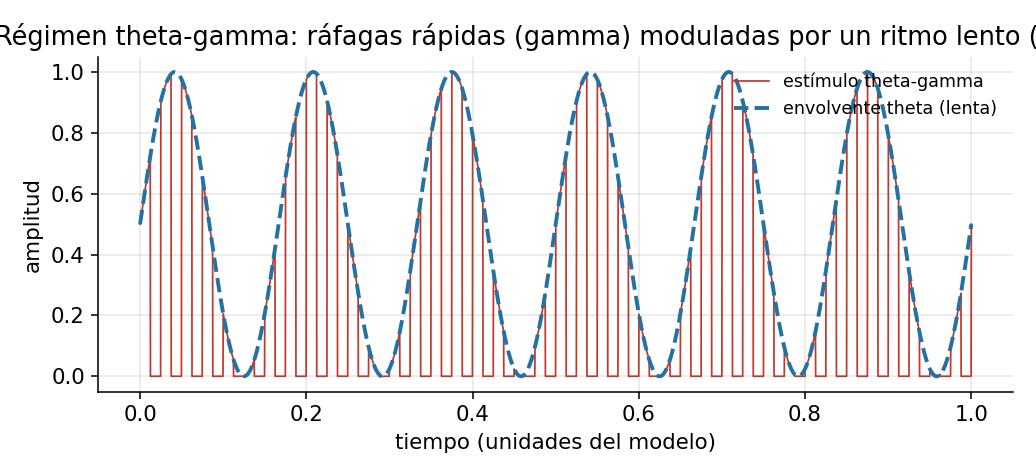
\includegraphics[width=0.75\linewidth]{fig_theta_gamma.png}
\caption{Régimen theta--gamma: ráfagas gamma rápidas cuya amplitud está modulada por
una envolvente theta lenta. La oscilación rápida es el lazo E--I de Wilson--Cowan; la
lenta la impone el estímulo/controlador. (figura del proyecto)}
\label{fig:theta_gamma}
\end{figure}

\paragraph{Por qué es el régimen propio de este proyecto.}
La Figura~\ref{fig:theta_gamma} es la ``firma'' que queremos producir e inducir. La
lectura mecanística en clave Wilson--Cowan es directa:
\begin{itemize}[nosep]
  \item El \textbf{gamma} lo genera el lazo E--I intrínseco del modelo (Sección~2).
  \item El \textbf{theta} lo impone una modulación lenta del \textbf{estímulo}: al
        hacer variar $P(t)$ (y/o $Q(t)$) con un ritmo lento, la población entra y sale
        del ciclo límite. Cuando el estímulo lento está ``arriba'', hay ráfaga gamma;
        cuando está ``abajo'', el gamma se apaga. El resultado es exactamente la
        envolvente theta sobre el gamma.
\end{itemize}
Es decir: theta--gamma \textbf{no} es un fenómeno externo que estudiamos por
curiosidad, es el \textbf{objetivo de control}. El controlador IMC (ver documentos de
la parte de control) manipula el estímulo lento para que el modelo identificado siga
una envolvente theta prescrita mientras el lazo E--I sigue produciendo gamma. Que el
estímulo sea del tipo on/off y $\geq 0$ no es casualidad: está pensado para ser
\emph{realizable con optogenética}, donde uno solo puede encender o apagar luz sobre
poblaciones excitatorias o inhibitorias, no aplicar corrientes negativas arbitrarias.

\begin{remark}
Este es el punto que cierra el arco del proyecto: la fragilidad para identificar
$w_{II}$ (el parámetro ``difícil'') vive en el detalle fino del lazo de inhibición,
pero el objetivo de control (seguir la envolvente theta) es una propiedad más gruesa
del sistema. Por eso se puede argumentar que la mala identificabilidad de $w_{II}$
\emph{no se propaga} al control theta--gamma.
\end{remark}

\section{Cómo se mide la actividad poblacional: EEG y LFP}

Para conectar el modelo con datos reales hay que entender qué se mide. Dos técnicas son
clave:
\begin{itemize}[nosep]
  \item \textbf{EEG (electroencefalograma):} electrodos en el cuero cabelludo. Mide el
        campo eléctrico generado por la actividad sincronizada de \emph{grandes}
        poblaciones corticales. Es no invasivo pero de baja resolución espacial: cada
        electrodo integra la actividad de millones de neuronas.
  \item \textbf{LFP (\emph{local field potential}):} un microelectrodo dentro del
        tejido. Mide el potencial extracelular \emph{local}, dominado por las
        corrientes sinápticas de la población cercana. Es invasivo pero mucho más
        local; es la señal más cercana a lo que modela una unidad de Wilson--Cowan.
\end{itemize}

\paragraph{Por qué $y = E - I$ es un buen proxy de potencial.}
Tanto EEG como LFP miden, en esencia, la \textbf{suma de corrientes} que las neuronas
inyectan al medio extracelular. Las poblaciones excitatoria e inhibitoria contribuyen
con \emph{signos opuestos} a ese potencial: las corrientes excitatorias y las
inhibitorias empujan el potencial extracelular en direcciones contrarias. Por eso la
combinación
$$y(t) = E(t) - I(t)$$
captura la \emph{diferencia neta} de actividad E--I, que es justamente lo que un
electrodo ``ve'' como fluctuación del campo. No pretende ser un modelo biofísico
detallado del electrodo; es un proxy simple y estándar en modelos de masa neuronal
\cite{deco2008dynamicbrain}. Consecuencia práctica para el proyecto: la \textbf{única
salida observable} es $y(t)=E-I$ (no medimos $E$ e $I$ por separado), y de esa señal
escalar hay que identificar los 10 parámetros. Esto es parte de por qué la
identificación es difícil, y por qué el espectro de $y(t)$ es lo que comparamos contra
las bandas theta y gamma.

\section{Función de los ritmos y relevancia clínica}

¿Por qué molestarse en controlar ritmos? Porque no son un epifenómeno: cumplen
funciones y, cuando se rompen, aparece patología.

\paragraph{Función.}
\begin{itemize}[nosep]
  \item \textbf{Comunicación neuronal:} la hipótesis de ``comunicación por coherencia''
        sostiene que dos regiones intercambian información de forma eficiente cuando sus
        oscilaciones gamma están en fase; el ritmo abre y cierra ventanas temporales de
        recepción \cite{buzsaki2006rhythms}.
  \item \textbf{Memoria de trabajo e hipocampo:} el acoplamiento theta--gamma se
        propone como un \emph{código}: cada ciclo de theta contiene varias ráfagas
        gamma, y cada ráfaga codifica un ítem distinto. Así el número de ráfagas gamma
        que entran en un ciclo theta pondría un límite a cuántos ítems mantenemos en
        memoria de trabajo \cite{lisman2013thetagamma}. El hipocampo, central en
        memoria y navegación, es el ejemplo canónico de este esquema.
\end{itemize}

\paragraph{Relevancia clínica.}
\begin{itemize}[nosep]
  \item \textbf{Epilepsia:} una crisis es, en buena medida, una sincronización
        patológica y excesiva de la actividad poblacional (un desbalance E/I que se
        desboca). Ya existen esquemas de control optogenético en lazo cerrado que
        detectan el inicio de la crisis y la abortan con luz
        \cite{krookmagnuson2013seizures}, lo cual es exactamente el tipo de escenario
        ``identificar + controlar'' que motiva este trabajo.
  \item \textbf{Parkinson:} se asocia a una sincronización patológica en banda beta en
        los ganglios basales; la estimulación cerebral profunda (DBS) busca justamente
        romper ese ritmo anómalo, y la elección de sus parámetros es un problema de
        diseño de estímulo \cite{kuncel2004dbs}.
\end{itemize}

En ambos casos la lógica es la misma que la del proyecto: si tengo un \emph{modelo}
confiable de la dinámica poblacional (Wilson--Cowan identificado a partir de $y=E-I$) y
un \emph{actuador} realizable (optogenética, on/off, $\geq 0$), puedo diseñar un
controlador que lleve al sistema al régimen deseado --- aquí, un theta--gamma sano ---
en lugar de dejarlo caer en el patológico. Ese es el hilo que une B3, este B4 y la
parte de control del paquete.

\begin{thebibliography}{9}
\bibitem{wilson1972}
H.~R. Wilson y J.~D. Cowan, ``Excitatory and inhibitory interactions in localized
populations of model neurons'', \emph{Biophysical Journal}, 12(1):1--24, 1972.
\bibitem{buzsaki2006rhythms}
G.~Buzsáki, \emph{Rhythms of the Brain}, Oxford University Press, 2006.
\bibitem{buzsaki2012gamma}
G.~Buzsáki y X.-J. Wang, ``Mechanisms of gamma oscillations'', \emph{Annual Review of
Neuroscience}, 35:203--225, 2012.
\bibitem{lisman2013thetagamma}
J.~E. Lisman y O.~Jensen, ``The theta-gamma neural code'', \emph{Neuron},
77(6):1002--1016, 2013.
\bibitem{deco2008dynamicbrain}
G.~Deco et al., ``The dynamic brain: from spiking neurons to neural masses and cortical
fields'', \emph{PLoS Computational Biology}, 4(8):e1000092, 2008.
\bibitem{krookmagnuson2013seizures}
E.~Krook-Magnuson et al., ``On-demand optogenetic control of spontaneous seizures in
temporal lobe epilepsy'', \emph{Nature Communications}, 4:1376, 2013.
\bibitem{kuncel2004dbs}
A.~M. Kuncel y W.~M. Grill, ``Selection of stimulus parameters for deep brain
stimulation'', \emph{Clinical Neurophysiology}, 115(11):2431--2441, 2004.
\end{thebibliography}

\end{document}
